
%(BEGIN_QUESTION)
% Copyright 2006, Tony R. Kuphaldt, released under the Creative Commons Attribution License (v 1.0)
% This means you may do almost anything with this work of mine, so long as you give me proper credit

Suppose a small rubber ball is floating inside the fluid of a hydraulic cylinder as shown below.  What will happen to the ball when a pushing force is exerted on the cylinder's rod?  What will happen to the ball when a pulling force is exerted on the rod?

$$\includegraphics[height=9cm]{i00143x01.eps}$$

\underbar{file i00143}
%(END_QUESTION)





%(BEGIN_ANSWER)

A pushing force on the rod will compress the rubber ball to a smaller diameter.  A pulling force will expand it to a larger diameter.

$$\includegraphics[width=15.5cm]{i00143x02.eps}$$

%(END_ANSWER)





%(BEGIN_NOTES)

A pushing force on the rod will compress the rubber ball to a smaller diameter, because the fluid pressure exerts a pushing force in all directions, including toward the ball's center.  A pulling force will expand the ball to a larger diameter because the vacuum (negative pressure) created will {\it pull} in all directions. 

$$\includegraphics[width=15.5cm]{i00143x03.eps}$$

%INDEX% Physics, static fluids: direction of force exerted by fluid pressure

%(END_NOTES)


